\cleardoublepage
% ==============================================================
\chapter*{Appendix A: qTrace -- Rapid quantitation of metabolically labeled sister peptides}
\markboth{Appendix A: qTrace -- Rapid quantitation of metabolically labeled sister peptides}{Appendix A: qTrace -- Rapid quantitation of metabolically labeled sister peptides}
\addcontentsline{toc}{chapter}{Appendix A: qTrace -- Rapid quantitation of metabolically labeled sister peptides}
% ==============================================================

In addition to identification, peptide and protein quantitation via mass 
spectrometry has become an important aspect of mass spectrometric analysis 
\citep{Kline2010, Schulze2010}. 
Various programs for peptide and protein quantitation in metabolically labeled 
samples have been published \citep{Han2001, Li2003, Saito2007, Park2008, 
Cox2008, Mortensen2010}, with different platform support and label handling 
capabilities. 
However, none of these tool provides operating-system independent support
for various metabolic labeling strategies.
To overcome this, qTrace, a novel quantitation software has been 
created in the scope of this thesis.
Like OMSSA, qTrace can be 
used within Proteomatic.
qTrace searches for the isotope envelopes of previously identified sister 
peptides in MS1 full scans and allows for various labeling strategies, 
including stable isotopic labeling by amino acids in cell culture (SILAC) 
and \textsuperscript{15}N labeling.

\section*{Quantitation workflow}

qTrace uses a list of peptides which have been previously identified via MS/MS
(`target peptides') and performs peptide quantitation based on the corresponding 
precursor ions in full scans.
Users may choose from a list of predefined labels or manually specify a 
labeling strategy using a syntax which accurately describes the label applied 
to the sample.
Labels can be defined by specifying certain isotopes such as `15N' or `13C'.
Combinations of multiple isotopes are possible. 
Isotopes may be followed by a labeling efficiency: `15N (0.994)'
indicates that 99.4\% of all nitrogen atoms in the labeled sample are 
\textsuperscript{15}N isotopes, and the remaining 0.06\% are 
\textsuperscript{14}N isotopes. 
Isotopes, or combinations thereof, may be prefixed with an 
amino acid scope that constrains isotopes to certain amino acids: 
`R 13C' indicates \textsuperscript{13}C atoms in all arginine residues (like for 
isotopes, multiple amino acids may be specified). 
To accommodate for the effect that labeled arginine residues may lead 
to labeled proline residues due to their shared amino acid biosynthesis pathways, 
variable labels may be defined by suffixing an amino acid with the star 
symbol: `RP* 13C' indicates heavy carbon atoms in all arginine residues 
and also variably in all proline residues, leading to $n$ additional labeled 
isotope envelopes, where $n$ is the number of proline residues in the target peptide.
Finally, an amino acid scope may be negated by using the caret symbol: 
`$\caret$R 15N' indicates \textsuperscript{15}N isotopes in all residues 
except arginine.

\section*{Abundance estimation}

qTrace offers two modes of abundance estimation: (a) a {\em fixed peak count} 
mode and (b) an {\em isotope envelope fitting} mode. 

In the {\em fixed peak count} mode, a fixed number of required isotope peaks $n$,
including the monoisotopic peak, is defined by the user.
qTrace calculates the {\em m/z} values of the respective isotope peaks 
\mbox{$A+0$} to $A+(n-1)$ for every unlabeled and labeled target peptide within 
a user-definable charge state range and stores these target peaks as 
`required present'. 
In addition, the $A-1$ peak of the light sister peptide is stored as 
`required absent', because its presence for one peptide would imply 
that its alleged $A+0$ peak might in fact be the $A+i$ peak of 
another peptide. 
The calculated {\em m/z} values are then matched to the observed {\em m/z} 
values within a user-defined precursor mass tolerance.
Whenever all presence and absence requirements are met for a certain unlabeled 
or labeled peptide, its abundance is estimated by summing the peak heights of 
all peaks stored as `required present'. 

Using the {\em isotope envelope fitting} mode, peak intensities are calculated in 
addition to the {\em m/z} values by predicting the shape of the 
isotope envelope from the elemental composition of every target peptide. 
Instead of defining a fixed number of isotope peaks per precursor ion, `required
present' peaks are defined using a relative intensity threshold in respect to the
highest peak of the predicted isotope envelope.
This leads to a variable `required isotope peak' count per peptide, depending on 
its elemental composition.
Typically, a relative intensity threshold of 50\% is used to define `required 
present' peaks. 

\begin{figure}
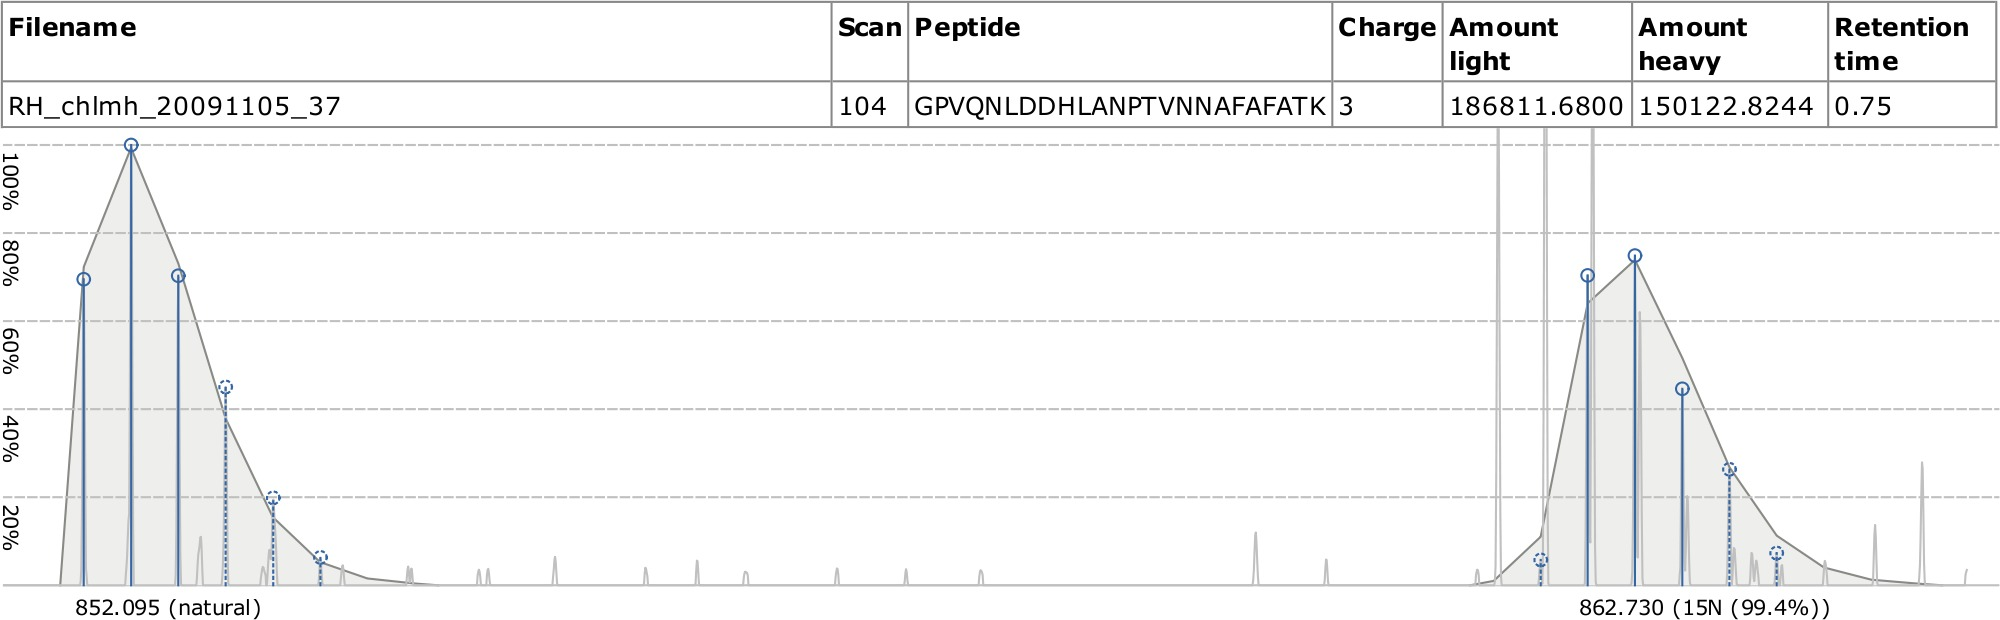
\includegraphics[width=\textwidth]{figures/qtrace-figure.jpg}
\caption{
    {\bf An example sister peptide pair from a 
    \textsuperscript{14}N/\textsuperscript{15}N labeled 
    {\em C. reinhardtii} sample as observed in a MS1 full scan. }
    {\em Required} peaks with a relative peak intensity of at least 50\% are 
    denoted by solid circled lines, {\em considered} peaks with a relative peak 
    intensity of at least 1\% are denoted by dashed circled lines. 
    The areas shaded in gray depict the theoretical isotope envelopes fitted to
    the observed {\em required} and {\em considerded} peaks and yield a light/heavy
    ratio of 1.24 for this scan.}
\label{fig:qtrace}
\end{figure}

All `required present' peaks have to be present in the spectrum for the peptide 
to be identified.
In addition, a variable number of `considered if present' peaks may be defined
via a second threshold (typically 1\%). 
All `required present' and `considered if present' {\em m/z} values are matched 
to the observed {\em m/z} values.
If all required peaks are present in the scan, the union of all `required' and
`considered' peaks is fitted to the theoretical isotope envelope, taking peak
heights into account.
A fitting error is determined and used to discard false matches.
Because the shape of the theoretical isotope envelope is taken into account, 
it is not necessary to check for the absence of the unlabeled $A-1$ peak.
The area under the fitted isotope envelope is then used as an estimate for
peptide abundance (see Fig.~\ref{fig:qtrace}).

\section*{Result compilation}

For demonstration purposes, the following experimental context is assumed:
\textsuperscript{14}N/\textsuperscript{15}N differentially labeled proteins from 
the unicellular green alga {\em Chlamydomonas reinhardtii} were mixed at equal 
protein concentration and fractionated by SDS-PAGE. After separation, protein 
bands were excised, digested with trypsin and analyzed by liquid chromatography 
coupled mass spectrometry.
Data evaluation of the resulting full and fragmentation scans was conducted via 
Proteomatic using OMSSA for identification and qTrace for quantitation. 

The output of qTrace is a list of peptide quantitation events in full scans.
Every quantitation event denotes unlabeled and labeled abundances of a peptide 
in a defined context (e.g. certain SDS-PAGE band and/or retention time),
at a certain charge state.
In the context of qTrace, the combination of peptide, band, and charge is called 
the {\em PBC combination} of a certain quantitation event.
Ratios are determined by dividing the sums of all unlabeled and labeled peptide
abundances within a PBC combination to accomodate for small retention time
shifts of sister peptides.
In addition, different PBC combinations can be regarded as independent observations 
of the peptide over retention time and a minimal PBC combination count can therefore 
be used as a filter criterion in a subsequent processing step.

The following filtering steps are provided by Proteomatic (see Fig.~\ref{fig:exp-setup}):

{\bf Add protein information.}
For every peptide quantitation event, the corresponding protein (or
protein group) is determined, and all quantitation events of peptides 
appearing in multiple proteins (or protein groups) are discarded.

\begin{figure*}
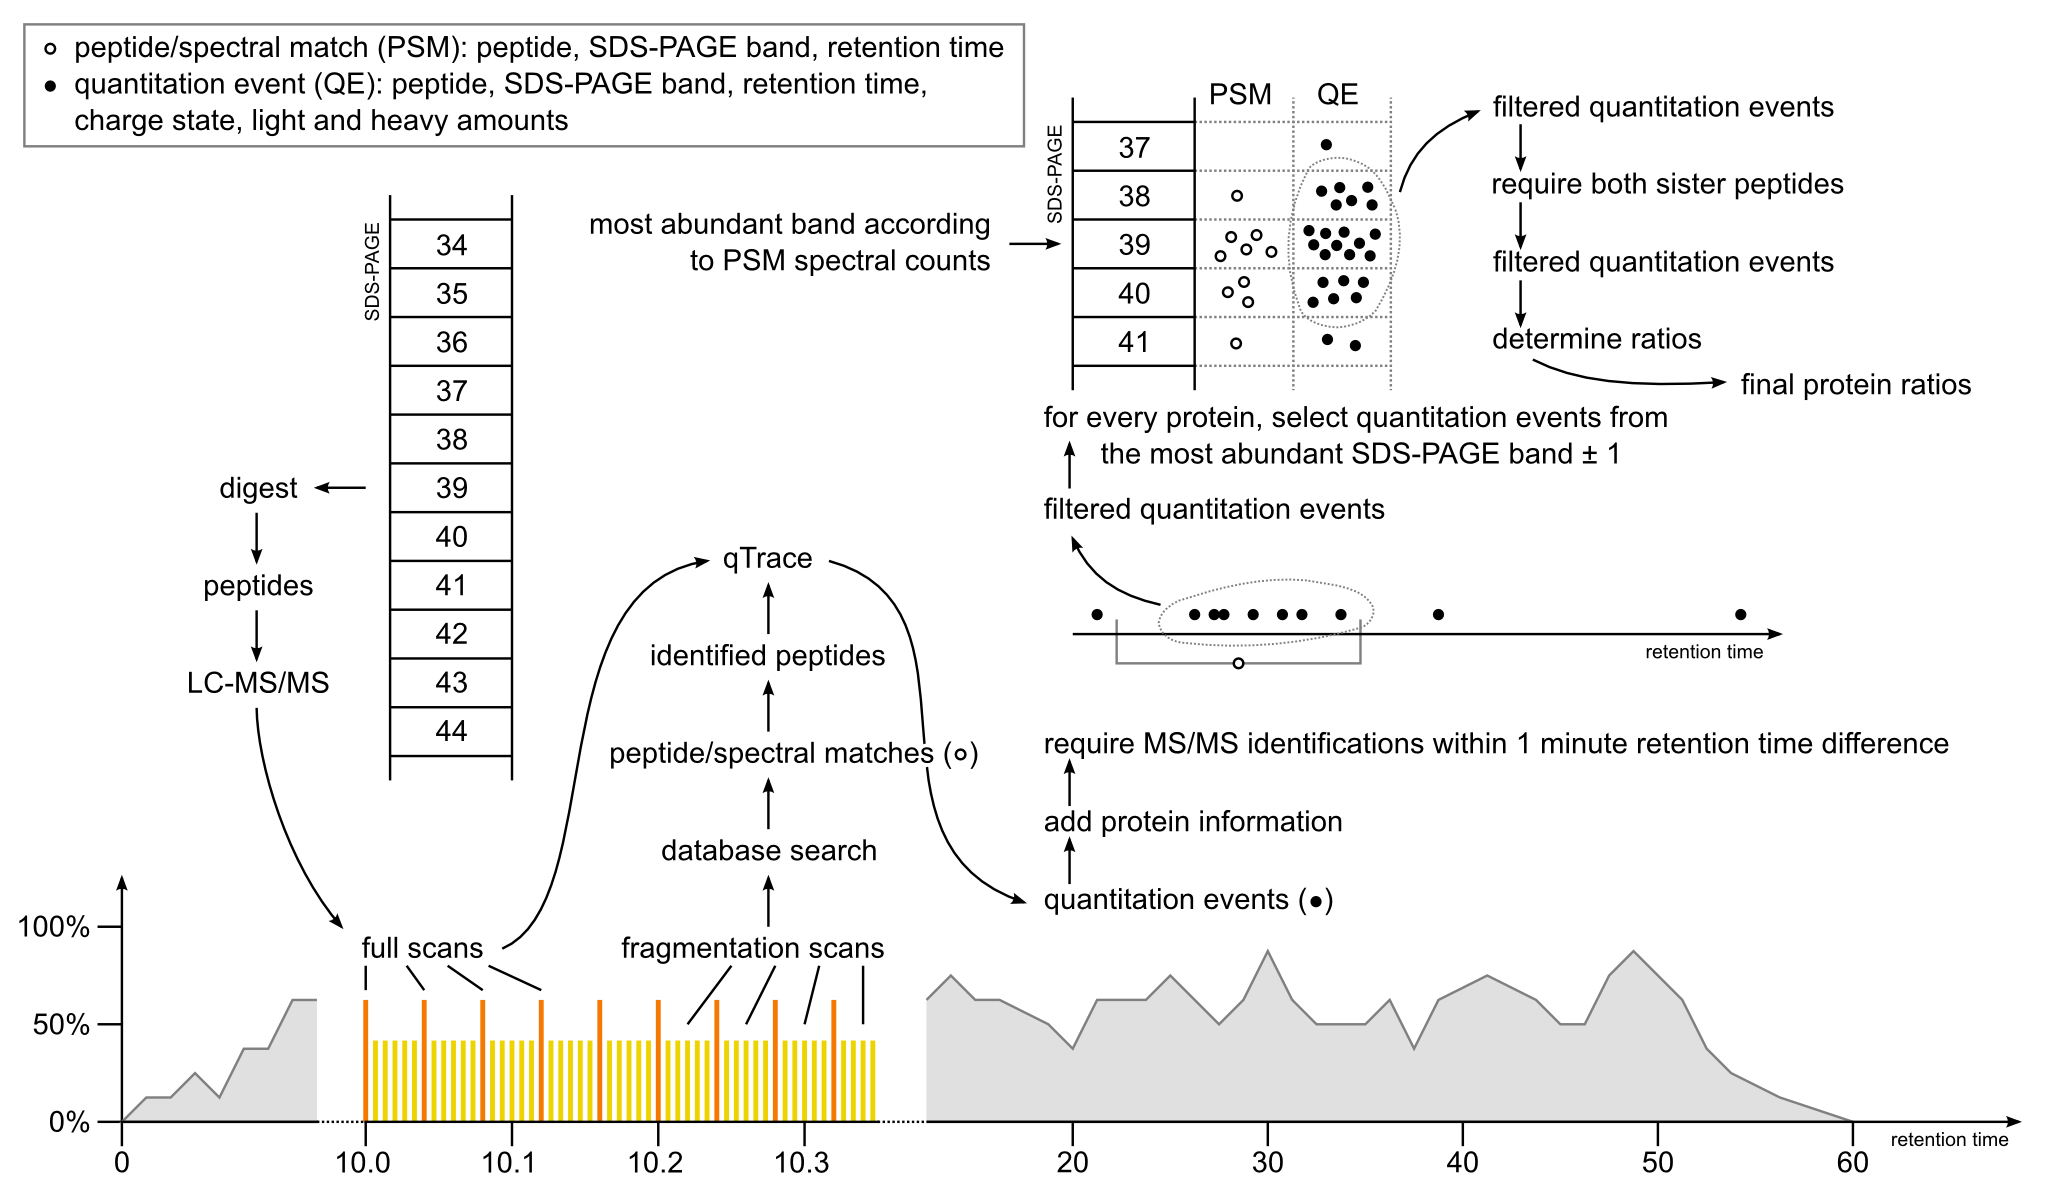
\includegraphics[width=\textwidth]{figures/exp-setup.jpg}
\caption{
    {\bf Depiction of the experimental workflow for protein identification and 
    quantitation. }
    Protein samples are subjected to two steps of separation: (a) SDS-PAGE, in 
    which each sample is fractionated into distinct bands, and (b) HPLC, which 
    separates the digested peptides from each SDS-PAGE band according to their 
    hydrophobicity. 
    The peptides eluting from the HPLC are measured using the {\em Big 5} 
    method which produces full scans and fragmentation scans in an interleaved 
    pattern. 
    While the fragmentation scans are used to identify peptides via a database 
    search (e. g. using OMSSA), the full scans are used by qTrace to quantify 
    the previously identified peptides using their light and heavy precursor 
    masses.
    The resulting quantitation events (QE) are then filtered in such a way
    that MS/MS identifications are required within a short retention time 
    difference. 
    The peptide quantitation events are compiled to protein quantitation events
    by determining which protein a peptide belongs to and discarding all events
    from ambiguous peptides.
    In addition, the spectral counts derived from the MS/MS identifications are 
    used to determine the SDS-PAGE band in which a protein has been must 
    abundantly identified in, and only quantitation events from this band 
    ($\pm$1) are accepted.
    Finally, the protein ratios are determined.
}
\label{fig:exp-setup}
\end{figure*}

{\bf Require MS/MS identifications.}
All quantitation events for which no MS/MS identification exists in the same 
SDS-PAGE band within a user-defined retention time difference (1 minute by 
default) are discarded. This filter corresponds to the separation of the 
tryptic peptides via liquid chromatography.

{\bf Pick most abundant SDS-PAGE band.}
For every protein, the SDS-PAGE band in which the protein has been identified 
in most abundantly is determined, and only quantitation events stemming from 
this band ($\pm$ a user-defined tolerance, typically 1) are discarded. This 
filter corresponds to the fractionation step via SDS-PAGE.

{\bf Require both sister peptides.}
Quantitation events in which only one of the sister peptides (labeled or 
unlabeled) could be quantified can be considered less reliable than quantitation 
events in which both sister peptides could be quantified.
This is because the missing peptide might have escaped detection due to a 
post-translation modification resulting in a different precursor mass. 
This filter rejects all quantitation events in which one sister peptide has 
been quantified with an abundance of zero.

{\bf Determine ratios.}
In all previous processing steps, only abundances have been determined and 
filtered. 
This step determines actual ratios by dividing the sums of unlabeled and 
labeled abundances within every PBC combination and then determining the final 
protein ratio as the mean (and standard deviation) of the individual PBC 
combination ratios.
A high number of PBC combination ratios is favorable because every PBC 
combination may be regarded as an independent observation of a sister peptide 
pair.
